\chapter{Quantum computing and cryptography
II}\label{21-Quantum-computing-and-}

Bell's Inequality is powerful demonstration that there is something very
strange going on with quantum mechanics. But could this ``strangeness''
be of any use to solve computational problems not directly related to
quantum systems? A priori, one could guess the answer is \emph{no}. In
1994 Peter Shor showed that one would be wrong:

\hypertarget{shorthm}{}
\begin{theorem}[Shor's Theorem] \label[theorem]{shorthm}

The map that takes an integer \(m\) into its prime factorization is
efficiently quantumly computable. Specifically, it can be computed using
\(O(\log^3 m)\) quantum gates.

\end{theorem}

This is an exponential improvement over the best known classical
algorithms, which as we mentioned before, take roughly
\(2^{\tilde{O(\log^{1/3}m)}}\) time.

We will now sketch the ideas behind Shor's algorithm. In fact, Shor
proved the following more general theorem:

\hypertarget{hiddengroupthm}{}
\begin{theorem}[Order Finding Algorithm] \label[theorem]{hiddengroupthm}

There is a quantum polynomial time algorithm that given a multiplicative
Abelian group \(\mathbb{G}\) and element \(g\in\mathbb{G}\) computes the
\emph{order} of \(g\) in the group.

\end{theorem}

Recall that the order of \(g\) in \(\mathbb{G}\) is the smallest
positive integer \(a\) such that \(g^a = 1\). By ``given a group'' we
mean that we can represent the elements of the group as strings of
length \(O(\log |\mathbb{G}|)\) and there is a
\(poly(\log|\mathbb{G}|)\) algorithm to perform multiplication in the
group.

\section{From order finding to factoring and discrete
log}\label{21-From-order-finding-to-}

The order finding problem allows not just to factor integers in
polynomial time, but also solve the discrete logarithm over arbitrary
Abelian groups, hereby showing that quantum computers will break not
just RSA but also Diffie Hellman and Elliptic Curve Cryptography. We
merely sketch how one reduces the factoring and discrete logarithm
problems to order finding: (see some of the sources above for the full
details)

\begin{itemize}
\item
  For \textbf{factoring}, let us restrict to the case \(m=pq\) for
  distinct \(p,q\). Recall that we showed that finding the size
  \((p-1)(q-1)=m-p-q+1\) of the group \(\Z^*_m\) is sufficient to
  recover \(p\) and \(q\). One can show that if we pick a few random
  \(x\)'s in \(\Z^*_m\) and compute their order, the least common
  multiplier of these orders is likely to be the group size.
\item
  For \textbf{discrete log} in a group \(\mathbb{G}\), if we get
  \(X=g^x\) and need to recover \(x\), we can compute the order of
  various elements of the form \(X^ag^b\). The order of such an element
  is a number \(c\) satisfying \(c(xa+b) = 0 \pmod{|\mathbb{G}|}\).
  Again, with a few random examples we will get a non trivial example
  (where \(c \neq 0 \pmod{|\mathbb{G}|}\) ) and be able to recover the
  unknown \(x\).
\end{itemize}

\section{Finding periods of a function: Simon's
Algorithm}\label{21-Finding-periods-of-a-f}

Let \(\mathbb{H}\) be some Abelian group with a group operation that
we'll denote by \(\oplus\), and \(f\) be some function mapping
\(\mathbb{H}\) to an arbitrary set (which we can encode as
\(\{0,1\}^*\)). We say that \(f\) has \emph{period \(h^*\)} for some
\(h^*\in\mathbb{H}\) if for every \(x,y \in \mathbb{H}\), \(f(x)=f(y)\)
if and only if \(y = x \oplus kh^*\) for some integer \(k\). Note that
if \(\mathbb{G}\) is some Abelian group, then if we define
\(\mathbb{H}=\Z_{|\mathbb{G}|}\), for every element \(g\in \mathbb{G}\),
the map \(f(a)=g^a\) is a periodic map over \(\mathbb{H}\) with period
the order of \(g\). So, finding the order of an item reduces to the
question of finding the period of a function.

How do we generally find the period of a function? Let us consider the
simplest case, where \(f\) is a function from \(\R\) to \(\R\) that is
\(h^*\) periodic for some number \(h^*\), in the sense that \(f\)
repeats itself on the intervals \([0,h^*]\), \([h^*,2h^*]\),
\([2h^*,3h^*]\), etc.. How do we find this number \(h^*\)? The key idea
would be to transform \(f\) from the \emph{time} to the \emph{frequency}
domain. That is, we use the \emph{Fourier transform} to represent \(f\)
as a sum of wave functions. In this representation wavelengths that
divide the period \(h^*\) would get significant mass, while wavelengths
that don't would likely ``cancel out''.

\begin{figure}
\centering
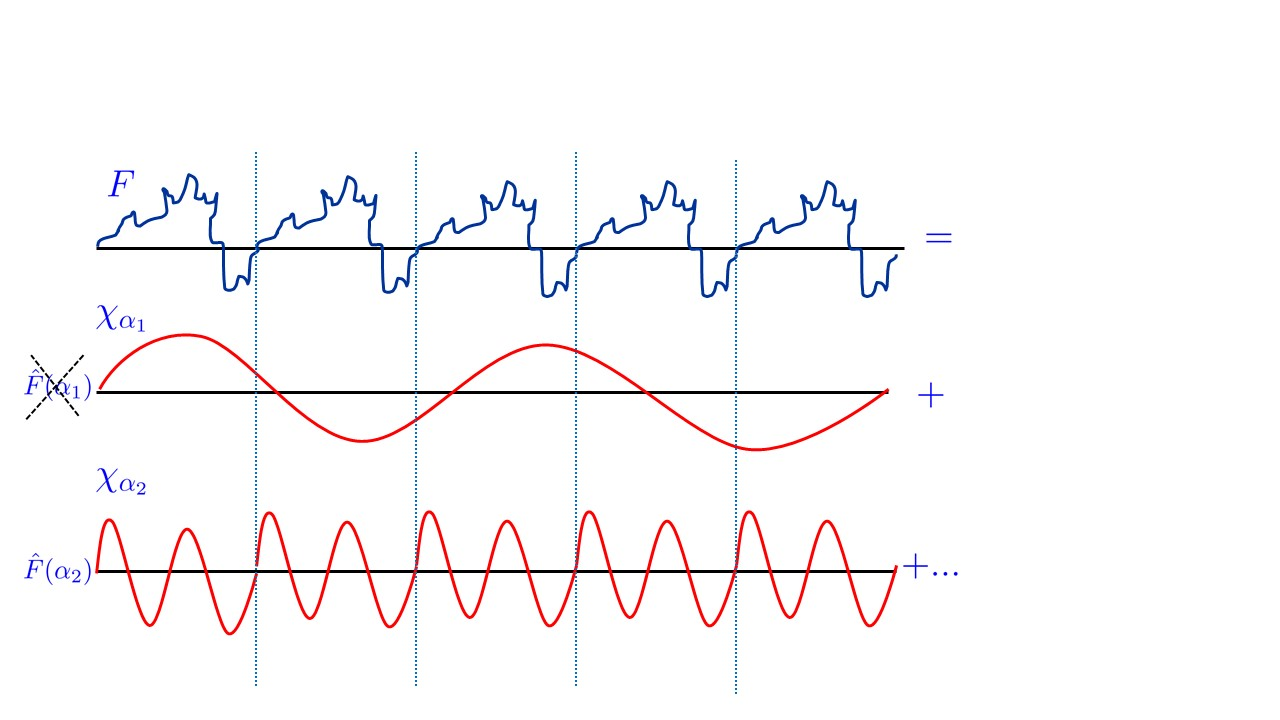
\includegraphics[width=\textwidth, height=0.25\paperheight, keepaspectratio]{../figure/quantum_fourier.jpg}
\caption{If \(f\) is a periodic function then when we represent it in
the Fourier transform, we expect the coefficients corresponding to
wavelengths that do not evenly divide the period to be very small, as
they would tend to ``cancel out''.}
\label{tmplabelfig}
\end{figure}

Similarly, the main idea behind Shor's algorithm is to use a tool known
as the \emph{quantum fourier transform} that given a circuit computing
the function \(f:\mathbb{H}\rightarrow\R\), creates a quantum state over
roughly \(\log |\mathbb{H}|\) qubits (and hence dimension
\(|\mathbb{H}|\)) that corresponds to the Fourier transform of \(f\).
Hence when we measure this state, we get a group element \(h\) with
probability proportional to the square of the corresponding Fourier
coefficient. One can show that if \(f\) is \(h^*\)-periodic then we can
recover \(h^*\) from this distribution.

Shor carried out this approach for the group \(\mathbb{H}=\Z^*_q\) for
some \(q\), but we will start be seeing this for the group
\(\mathbb{H} = \{0,1\}^n\) with the XOR operation. This case is known as
\emph{Simon's algorithm} (given by Dan Simon in 1994) and actually
preceded (and inspired) Shor's algorithm:

\hypertarget{simonsthm}{}
\begin{theorem}[Simon's Algorithm] \label[theorem]{simonsthm}

If \(f:\{0,1\}^n\rightarrow\{0,1\}^*\) is polynomial time computable and
satisfies the property that \(f(x)=f(y)\) iff \(x\oplus y = h^*\) then
there exists a quantum polynomial-time algorithm that outputs a random
\(h\in \{0,1\}^n\) such that \(\langle h,h^* \rangle=0 \pmod{2}\).

\end{theorem}

Note that given \(O(n)\) such samples, we can recover \(h^*\) with high
probability by solving the corresponding linear equations.

\begin{proof} \label[proof]{21-Let-ensuremathmathitHA}

Let \(\ensuremath{\mathit{HAD}}\) be the \(2\times 2\) unitary matrix
corresponding to the one qubit operation
\(|0\rangle \mapsto \tfrac{1}{\sqrt{2}}(|0\rangle+|1\rangle)\) and
\(|1\rangle \mapsto \tfrac{1}{\sqrt{2}}(|0\rangle-|1\rangle)\) or
\(|a\rangle\mapsto \tfrac{1}{\sqrt{2}}(|0\rangle+(-1)^a|1\rangle)\).
Given the state \(|0^{n+m\rangle}\) we can apply this map to each one of
the first \(n\) qubits to get the state
\(2^{-n/2}\sum_{x\in\{0,1\}^n}|x\rangle|0^m\rangle\) and then we can
apply the gates of \(f\) to map this to the state
\(2^{-n/2}\sum_{x\in\{0,1\}^n}|x\rangle|f(x)\rangle\) now suppose that
we apply this operation again to the first \(n\) qubits then we get the
state
\(2^{-n}\sum_{x\in\{0,1\}^n}\prod_{i=1}^n(|0\rangle+(-1)^{x_i}|1\rangle)|f(x)\rangle\)
which if we open up each one of these product and look at all \(2^n\)
choices \(y\in\{0,1\}^n\) (with \(y_i=0\) corresponding to picking
\(|0\rangle\) and \(y_i=1\) corresponding to picking \(|1\rangle\) in
the \(i^{th}\) product) we get
\(2^{-n}\sum_{x\in\{0,1\}^n}\sum_{y\in\{0,1\}^n}(-1)^{\langle x,y \rangle}|y\rangle|f(x)\rangle\).
Now under our assumptions for every particular \(z\) in the image of
\(f\), there exist exactly two preimages \(x\) and \(x\oplus h^*\) such
that \(f(x)=f(x+h^*)=z\). So, if \(\langle y,h^* \rangle=0 \pmod{2}\),
we get that
\((-1)^{\langle x,y \rangle}+(-1)^{\langle x,y+h^* \rangle}=2\) and
otherwise we get
\((-1)^{\langle x,y \rangle}+(-1)^{\langle x,y+h^* \rangle}=0\).
Therefore, if measure the state we will get a pair \((y,z)\) such that
\(\langle y,h^* \rangle=0 \pmod{2}\). QED

\end{proof}

Simon's algorithm seems to really use the special bit-wise structure of
the group \(\{0,1\}^n\), so one could wonder if it has any relevance for
the group \(\Z^*_m\) for some exponentially large \(m\). It turns out
that the same insights that underlie the well known Fast Fourier
Transform (FFT) algorithm can be used to essentially follow the same
strategy for this group as well.

\section{From Simon to Shor}\label{21-From-Simon-to-Shor}

(Note: The presentation here is adapted from the quantum computing
chapter in my textbook with Arora.)

We now describe how to achieve Shor's algorithm for order finding. We
will not do this for a general group but rather focus our attention on
the group \(\Z^*_{\ell}\) for some number \(\ell\) which is the case of
interest for integer factoring and the discrete logarithm modulo primes
problems.

That is, we prove the following theorem:

\hypertarget{shortwothm}{}
\begin{theorem}[Shor's Algorithm, restated] \label[theorem]{shortwothm}

For every \(\ell\) and \(a\in\Z^*_\ell\), there is a quantum
\(poly(log \ell)\) algorithm to find the order of \(a\) in
\(\Z^*_\ell\).

\end{theorem}

The idea is similar to Simon's algorithm. We consider the map
\(x \mapsto a^x (\mod \ell)\) which is a periodic map over \(\Z_m\)
where \(m=|\Z^*_\ell|\) with period being the order of \(a\).\\
To find the period of this map we will now need to perform a
\emph{Quantum Fourier Transform (QFT)} over the group \(\Z_m\) instead
of \(\{0,1\}^n\). This is a quantum algorithm that takes a register from
some arbitrary state \(f \in \mathbb{C}^{m}\) into a state whose vector
is the Fourier transform \(\hat{f}\) of \(f\). The QFT takes only
\(O(\log^2 m)\) elementary steps and is thus very efficient. Note that
we cannot say that this algorithm ``computes'' the Fourier transform,
since the transform is stored in the amplitudes of the state, and as
mentioned earlier, quantum mechanics give no way to ``read out'' the
amplitudes per se. The only way to get information from a quantum state
is by \emph{measuring} it, which yields a single basis state with
probability that is related to its amplitude. This is hardly
representative of the entire Fourier transform vector, but sometimes (as
is the case in Shor's algorithm) this is enough to get highly
non-trivial information, which we do not know how to obtain using
classical (non-quantum) computers.

\subsection{The Fourier transform over
\(\Z_m\)}\label{21-The-Fourier-transform-}

We now define the Fourier transform over \(\Z_m\) (the group of integers
in \(\{0,\ldots,m-1\}\) with addition modulo \(m\)). We give a
definition that is specialized to the current context. For every vector
\(f\in\mathbb{C}^m\), the \emph{Fourier transform of \(f\)} is the
vector \(\hat{f}\) where the \(x^{th}\) coordinate of \(\hat{f}\) is
defined as\footnote{In the context of Fourier transform it is customary
  and convenient to denote the \(x^{th}\) coordinate of a vector \(f\)
  by \(f(x)\) rather than \(f_x\).}

\(\hat{f}(x) = \tfrac{1}{\sqrt{m}}\sum_{y\in\Z_m} f(x)\omega^{xy}\)

where \(\omega = e^{2\pi i/m}\).

The Fourier transform is simply a representation of \(f\) in the
\emph{Fourier basis} \(\{ \chi_x \}_{x \in \Z_m}\), where \(\chi_x\) is
the vector/function whose \(y^{th}\) coordinate is
\(\tfrac{1}{\sqrt{m}\omega^{xy}}\). Now the inner product of any two
vectors \(\chi_x,\chi_z\) in this basis is equal to
\begin{equation*}
\langle \chi_x,\chi_z \rangle = \tfrac{1}{m}\sum_{y\in\Z_m} \omega^{xy} \overline{\omega^{zy}} = \tfrac{1}{m}\sum_{y\in\Z_m} \omega^{(x-z)y}  \;.
\end{equation*}
But if \(x=z\) then \(\omega^{(x-z)}=1\) and hence this sum is equal to
\(1\). On the other hand, if \(x \neq z\), then this sum is equal to
\(\tfrac{1}{m} \tfrac{1 -\omega^{(x-y)m}}{1-\omega^{x-y}}= \tfrac{1}{m}\tfrac{1-1}{1-\omega^{x-y}}=0\)
using the formula for the sum of a geometric series. In other words,
this is an \emph{orthonormal} basis which means that the Fourier
transform map \(f \mapsto \hat{f}\) is a \emph{unitary} operation.

What is so special about the Fourier basis? For one thing, if we
identify vectors in \(\mathbb{C}^m\) with functions mapping \(\Z_m\) to
\(\mathbb{C}\), then it's easy to see that every function \(\chi\) in
the Fourier basis is a \emph{homomorphism} from \(\Z_m\) to
\(\mathbb{C}\) in the sense that \(\chi(y+z)= \chi(y)\chi(z)\) for every
\(y,z \in \Z_m\). Also, every function \(\chi\) is \emph{periodic} in
the sense that there exists \(r\in \Z_m\) such that
\(\chi(y+r)=\chi(z)\) for every \(y\in \Z_m\) (indeed if
\(\chi(y) = \omega^{xy}\) then we can take \(r\) to be \(\ell/x\) where
\(\ell\) is the least common multiple of \(x\) and \(m\)). Thus,
intuitively, if a function \(f:\Z_m\rightarrow\mathbb{C}\) is itself
periodic (or roughly periodic) then when representing \(f\) in the
Fourier basis, the coefficients of basis vectors with periods agreeing
with the period of \(f\) should be large, and so we might be able to
discover \(f\)'s period from this representation. This does turn out to
be the case, and is a crucial point in Shor's algorithm.

\subsubsection{Fast Fourier Transform.}\label{21-Fast-Fourier-Transform}

Denote by \(\ensuremath{\mathit{FT}}_m\) the operation that maps every
vector \(f\in\mathbb{C}^m\) to its Fourier transform \(\hat{f}\). The
operation \(\ensuremath{\mathit{FT}}_m\) is represented by an
\(m\times m\) matrix whose \((x,y)\)th entry is \(\omega^{xy}\). The
trivial algorithm to compute it takes \(m^2\) operations. The famous
\emph{Fast Fourier Transform} (FFT) algorithm computes the Fourier
transform in \(O(m\log m)\) operations. We now sketch the idea behind
the FFT algorithm as the same idea is used in the \emph{quantum} Fourier
transform algorithm.

Note that

\(\hat{f}(x) = \tfrac{1}{\sqrt{m}}\sum_{y\in\Z_m} f(y)\omega^{xy} =\)

\(\tfrac{1}{\sqrt{m}}\sum_{y\in\Z_m,y \;even} f(y)\omega^{-2x(y/2)} + \omega^x\tfrac{1}{\sqrt{m}}\sum_{y\in\Z_m,y \;odd} f(y)\omega^{2x(y-1)/2} \;.\)

Now since \(\omega^2\) is an \(m/2\)th root of unity and
\(\omega^{m/2}=-1\), letting \(W\) be the \(m/2 \times m/2\) diagonal
matrix with diagonal entries \(\omega^0,\ldots,\omega^{m/2-1}\), we get
that

\(\ensuremath{\mathit{FT}}_m(f)_{low} = \ensuremath{\mathit{FT}}_{m/2}(f_{even}) + W \ensuremath{\mathit{FT}}_{m/2}(f_{odd})\)

\(\ensuremath{\mathit{FT}}_m(f)_{high} = \ensuremath{\mathit{FT}}_{m/2}(f_{even}) - W \ensuremath{\mathit{FT}}_{m/2}(f_{odd})\)

where for an \(m\)-dimensional vector \(\vec{v}\), we denote by
\(\vec{v}_{even}\) (resp. \(\vec{v}_{odd}\)) the \(m/2\)-dimensional
vector obtained by restricting \(\vec{v}\) to the coordinates whose
indices have least significant bit equal to \(0\) (resp. \(1\)) and by
\(\vec{v}_{low}\) (resp. \(\vec{v}_{high}\)) the restriction of
\(\vec{v}\) to coordinates with most significant bit \(0\) (resp.
\(1\)).

The equations above are the crux of the divide-and-conquer idea of the
FFT algorithm, since they allow to replace a size-\(m\) problem with two
size-\(m/2\) subproblems, leading to a recursive time bound of the form
\(T(m) = 2T(m/2) + O(m)\) which solves to \(T(m)=O(m\log m)\).

\subsection{Quantum Fourier Transform over
\(\Z_m\)}\label{21-Quantum-Fourier-Transf}

The \emph{quantum Fourier transform} is an algorithm to change the state
of a quantum register from \(f \in \mathbb{C}^m\) to its Fourier
transform \(\hat{f}\).

\hypertarget{quantumftthm}{}
\begin{theorem}[Quantum Fourier Transform (Bernstein-Vazirani)] \label[theorem]{quantumftthm}

For every \(m\) and \(m =2^m\) there is a quantum algorithm that uses
\(O(m^2)\) elementary quantum operations and transforms a quantum
register in state \(f = \sum_{x\in\Z_m} f(x)|x\rangle\) into the state
\(\hat{f}= \sum_{x\in\Z_m} \hat{f}(x) |x\rangle\), where
\(\hat{f}(x) = \tfrac{1}{\sqrt{m}} \sum_{y\in \Z_m} \omega^{xy}f(x)\).

\end{theorem}

The crux of the algorithm is the FFT equations, which allow the problem
of computing \(\ensuremath{\mathit{FT}}_m\), the problem of size \(m\),
to be split into two identical subproblems of size \(m/2\) involving
computation of \(\ensuremath{\mathit{FT}}_{m/2}\), which can be carried
out recursively using the same elementary operations. (Aside: Not every
divide-and-conquer classical algorithm can be implemented as a fast
quantum algorithm; we are really using the structure of the problem
here.)

We now describe the algorithm and the state, neglecting normalizing
factors.

\begin{enumerate}
\def\labelenumi{\arabic{enumi}.}
\item
  \emph{initial state:} \(f= \sum_{x\in\Z_m} f(x)|x\rangle\)
\item
  Recursively run \(\ensuremath{\mathit{FT}}_{m/2}\) on \(m-1\) most
  significant qubits (state:
  \((\ensuremath{\mathit{FT}}_{m/2}f_{even})|0\rangle + (\ensuremath{\mathit{FT}}_{m/2}f_{odd})|1\rangle\))
\item
  If LSB is \(1\) then compute \(W\) on \(m-1\) most significant qubits
  (see below). (state :
  \((\ensuremath{\mathit{FT}}_{m/2}f_{even})|0\rangle + (W \ensuremath{\mathit{FT}}_{m/2}f_{odd})|1\rangle\))
\item
  Apply Hadmard gate \(H\) to least significant qubit. (state:
  \((\ensuremath{\mathit{FT}}_{m/2}f_{even})(|0\rangle+|1\rangle)\)
  \(+\)
  \((W \ensuremath{\mathit{FT}}_{m/2}f_{odd})(|0\rangle-|1\rangle) =\)
  \((\ensuremath{\mathit{FT}}_{m/2}f_{even}+ W \ensuremath{\mathit{FT}}_{m/2}f_{odd})|0\rangle + (\ensuremath{\mathit{FT}}_{m/2}f_{even}-W \ensuremath{\mathit{FT}}_{m/2}f_{odd})|1\rangle\))
\item
  Move LSB to the most significant position (state:
  \(|0\rangle(\ensuremath{\mathit{FT}}_{m/2}f_{even}+ W \ensuremath{\mathit{FT}}_{m/2}f_{odd}) + |1\rangle(\ensuremath{\mathit{FT}}_{m/2}f_{even}- W \ensuremath{\mathit{FT}}_{m/2}f_{odd}) = \hat{f}\))
\end{enumerate}

The transformation \(W\) on \(m-1\) qubits can be defined by
\(|x\rangle \mapsto \omega^x = \omega^{\sum_{i=0}^{m-2} 2^ix_i}\) (where
\(x_i\) is the \(i^{th}\) qubit of \(x\)). It can be easily seen to be
the result of applying for every \(i\in \{ 0,\ldots,m-2\}\) the
following elementary operation on the \(i^{th}\) qubit of the register:

\(|0\rangle \mapsto |0\rangle\) and
\(|1\rangle \mapsto \omega^{2^i}|1\rangle\).

The final state is equal to \(\hat{f}\) by the FFT equations (we leave
this as an exercise)

\section{Shor's Order-Finding
Algorithm.}\label{21-Shors-Order-Finding-Al}

We now present the central step in Shor's factoring algorithm: a quantum
polynomial-time algorithm to find the \emph{order} of an integer \(a\)
modulo an integer \(\ell\).

\hypertarget{orderdinfindrestatethm}{}
\begin{theorem}[Order finding algorithm, restated] \label[theorem]{orderdinfindrestatethm}

There is a polynomial-time quantum algorithm that on input \(A,N\)
(represented in binary) finds the smallest \(r\) such that
\(A^r=1 \pmod{N}\).

\end{theorem}

Let \(t=\ceil{5\log (A+N)}\). Our register will consist of
\(t+polylog(N)\) qubits. Note that the function
\(x \mapsto A^x \pmod{N}\) can be computed in \(polylog(N)\) time and so
we will assume that we can compute the map
\(|x\rangle|y\rangle \mapsto |x\rangle|y\oplus (A^x \pmod{N\rangle)}\)
(where we identify a number \(X \in \{ 0,\ldots,N-1\}\) with its
representation as a binary string of length \(\log N\)).\footnote{To
  compute this map we may need to extend the register by some additional
  \(polylog(N)\) many qubits, but we can ignore them as they will always
  be equal to zero except in intermediate computations.} Now we describe
the order-finding algorithm. It uses a tool of elementary number theory
called \emph{continued fractions} which allows us to approximate (using
a classical algorithm) an arbitrary real number \(\alpha\) with a
rational number \(p/q\) where there is a prescribed upper bound on \(q\)
(see below)

We now describe the algorithm and the state, this time \emph{including}
normalizing factors.

\begin{enumerate}
\def\labelenumi{\arabic{enumi}.}
\item
  Apply Fourier transform to the first \(m\) bits. (state:
  \(\tfrac{1}{\sqrt{m}}\sum_{x\in\Z_m}|x\rangle)|0^n\rangle\))
\item
  Compute the transformation
  \(|x\rangle|y\rangle \mapsto |x\rangle|y \oplus (A^x \pmod{N\rangle)}\).
  (state:
  \(\tfrac{1}{\sqrt{m}}\sum_{x\in\Z_m} |x\rangle|A^x \pmod{N\rangle}\))
\item
  Measure the second register to get a value \(y_0\). (state:
  \(\tfrac{1}{\sqrt{K}}\sum_{\ell=0}^{K-1}|x_0 + \ell r\rangle|y_0\rangle\)
  where \(x_0\) is the smallest number such that
  \(A^{x_0} = y_0 \pmod{N}\) and \(K= \floor{(m-1-x_0)/r}\).)
\item
  Apply the Fourier transform to the first register. (state:
  \(\tfrac{1}{\sqrt{m}\sqrt{K}} \left(\sum_{x\in\Z_n}\sum_{\ell=0}^{K-1} \omega^{(x_0+\ell r)x}|x\rangle \right) |y_0\rangle\))
\end{enumerate}

In the analysis, it will suffice to show that this algorithm outputs the
order \(r\) with probability at least \(\Omega(1/\log N)\) (we can
always amplify the algorithm's success by running it several times and
taking the smallest output).

\subsection{Analysis: the case that
\(r|m\)}\label{21-Analysis-the-case-that}

We start by analyzing the algorithm in the case that \(m = rc\) for some
integer \(c\). Though very unrealistic (remember that \(m\) is a power
of \(2\)!) this gives the intuition why Fourier transforms are useful
for detecting periods.

\paragraph{Claim:} In this case the value \(x\) measured will be equal
to \(ac\) for a random \(a \in \{0,\ldots,r-1\}\).

The claim concludes the proof since it implies that \(x/m = a/r\) where
\(a\) is random integer less than \(r\). Now for every \(r\), at least
\(\Omega(r/\log r)\) of the numbers in \([r-1]\) are co-prime to \(r\).
Indeed, the prime number theorem says that there at least this many
primes in this interval, and since \(r\) has at most \(\log r\) prime
factors, all but \(\log r\) of these primes are co-prime to \(r\). Thus,
when the algorithm computes a rational approximation for \(x/m\), the
denominator it will find will indeed be \(r\).

To prove the claim, we compute for every \(x \in \Z_m\) the absolute
value of \(|x\rangle\)'s coefficient before the measurement. Up to some
normalization factor this is

\(\left| \sum_{\ell=0}^{c-1} \omega^{(x_0+\ell r)x} \right| = \left| \omega^{x_0c'c} \right| \left| \sum_{\ell=0}^{c-1} \omega^{r\ell x} \right| = 1 \cdot \left| \sum_{\ell=0}^{c-1} \omega^{r\ell x} \right| \;.\)

If \(c\) does not divide \(x\) then \(\omega^r\) is a \(c^{th}\) root of
unity, so \(\sum_{\ell=0}^{c-1} w^{r \ell x} =0\) by the formula for
sums of geometric progressions. Thus, such a number \(x\) would be
measured with zero probability. But if \(x = cj\) then
\(\omega^{r\ell x} = w^{r c j \ell} = \omega^{Mj} = 1\), and hence the
amplitudes of all such \(x\)'s are equal for all
\(j \in \{0, 2, \ldots, r-1\}\).

\subsubsection{The general case}\label{21-The-general-case}

In the general case, where \(r\) does not necessarily divide \(m\), we
will not be able to show that the measured value \(x\) satisfies
\(m | xr\). However, we will show that with \(\Omega(1/\log r)\)
probability, \textbf{(1)} \(xr\) will be ``almost divisible'' by \(m\)
in the sense that \(0 \leq xr \pmod{m} < r/10\) and \textbf{(2)}
\(\floor{xr/m}\) is coprime to \(r\).

Condition \textbf{(1)} implies that \(|xr - cM| < r/10\) for
\(c=\floor{xr/m}\). Dividing by \(rM\) gives
\(\left| \frac{x}{m} - \tfrac{c}{r} \right| < \tfrac{1}{10M}\).
Therefore, \(\tfrac{c}{r}\) is a rational number with denominator at
most \(N\) that approximates \(\frac{x}{m}\) to within
\(1/(10M) < 1/(4N^4)\). It is not hard to see that such an approximation
is unique (again left as an exercise) and hence in this case the
algorithm will come up with \(c/r\) and output the denominator \(r\).

Thus all that is left is to prove the next two lemmas. The first shows
that there are \(\Omega(r/\log r)\) values of \(x\) that satisfy the
above two conditions and the second shows that each is measured with
probability \(\Omega((1/\sqrt{r})^2) =\Omega(1/r)\).

\paragraph{Lemma 1:} There exist \(\Omega(r/\log r)\) values
\(x \in \Z_m\) such that:

\begin{enumerate}
\def\labelenumi{\arabic{enumi}.}
\item
  \(0 < xr \pmod{m} < r/10\)
\item
  \(\floor{xr/m}\) and \(r\) are coprime
\end{enumerate}

\paragraph{Lemma 2:} If \(x\) satisfies \(0 < xr \pmod{m} < r/10\) then,
before the measurement in the final step of the order-finding algorithm,
the coefficient of \(|x\rangle\) is at least
\(\Omega(\tfrac{1}{\sqrt{r}})\).

\paragraph{Proof of Lemma 1} We prove the lemma for the case that \(r\)
is coprime to \(m\), leaving the general case to the reader. In this
case, the map \(x \mapsto rx \pmod{m}\) is a permutation of \(\Z^*_m\).
There are at least \(\Omega(r/\log r)\) numbers in \([1..r/10]\) that
are coprime to \(r\) (take primes in this range that are not one of
\(r\)'s at most \(\log r\) prime factors) and hence \(\Omega(r/\log r)\)
numbers \(x\) such that \(rx \pmod{m} = xr - \floor{xr/m}m\) is in
\([1..r/10]\) and coprime to \(r\). But this means that \(\floor{rx/m}\)
can not have a nontrivial shared factor with \(r\), as otherwise this
factor would be shared with \(rx \pmod{m}\) as well.

\paragraph{Proof of Lemma 2:} Let \(x\) be such that
\(0 < xr \pmod{m} < r/10\). The absolute value of \(|x\rangle\)'s
coefficient in the state before the measurement is
\begin{equation*}
\tfrac{1}{\sqrt{K}\sqrt{m}}\left| \sum_{\ell=0}^{K-1} \omega^{\ell r x} \right| \;,
\end{equation*}
where \(K = \floor{(m-x_0-1)/r}\). Note that
\(\tfrac{m}{2r} < K < \tfrac{m}{r}\) since \(x_0 < N \ll m\).

Setting \(\beta=\omega^{rx}\) (note that since \(m \not| rx\),
\(\beta \neq 1\)) and using the formula for the sum of a geometric
series, this is at least
\(\tfrac{\sqrt{r}}{2M}\left| \tfrac{1 - \beta^{\ceil{m/r}}}{1-\beta} \right| = \tfrac{\sqrt{r}}{2M}\tfrac{\sin(\theta\ceil{m/r}/2)}{\sin(\theta/2)} \;,\)
where \(\theta=\tfrac{rx \pmod{m}}{m}\) is the angle such that
\(\beta = e^{i\theta}\) (see Figure~{[}quantum:fig:theta{]} for a proof
by picture of the last equality). Under our assumptions
\(\ceil{m/r}\theta<1/10\) and hence (using the fact that
\(\sin \alpha \sim \alpha\) for small angles \(\alpha\)), the
coefficient of \(x\) is at least
\(\tfrac{\sqrt{r}}{4M}\ceil{m/r} \geq \tfrac{1}{8\sqrt{r}}\)

This completes the proof of \cref{orderdinfindrestatethm}.

\section{Rational approximation of real
numbers}\label{21-Rational-approximation}

In many settings, including Shor's algorithm, we are given a real number
in the form of a program that can compute its first \(t\) bits in
\(poly(t)\) time. We are interested in finding a close approximation to
this real number of the form \(a/b\), where there is a prescribed upper
bound on \(b\). Continued fractions is a tool in number theory that is
useful for this.

A \emph{continued fraction} is a number of the following form:
\(a_0 + \frac{1}{a_1 + \frac{1}{a_2 + \tfrac{1}{a_3 + \ldots}} }\) for
\(a_0\) a non-negative integer and \(a_1,a_2,\ldots\) positive integers.

Given a real number \(\alpha>0\), we can find its representation as an
\emph{infinite} fraction as follows: split \(\alpha\) into the integer
part \(\floor{\alpha}\) and fractional part \(\alpha - \floor{\alpha}\),
find recursively the representation \(R\) of
\(1/(\alpha - \floor{\alpha})\), and then write
\begin{equation*}
\alpha = \floor{\alpha} + \frac{1}{R} \;.
\end{equation*}
If we continue this process for \(n\) steps, we get a rational number,
denoted by \([a_0,a_1,\ldots,a_n]\), which can be represented as
\(\tfrac{p_n}{q_n}\) with \(p_n,q_n\) coprime. The following facts can
be proven using induction:

\begin{itemize}
\item
  \(p_0=a_0, q_0 =1\) and for every \(n>1\),
  \(p_n = a_np_{n-1} + p_{n-2}\), \(q_n = a_nq_{n-1} + q_{n-2}\).
\item
  \(\tfrac{p_n}{q_n} - \tfrac{p_{n-1}}{q_{n-1}} = \tfrac{(-1)^{n-1}}{q_nq_{n-1}}\)
\end{itemize}

Furthermore, it is known that
\(\Bigl|\tfrac{p_n}{q_n} - \alpha\Bigl| < \tfrac{1}{q_nq_{n+1}} (*)\)
which implies that \(\tfrac{p_n}{q_n}\) is the \emph{closest} rational
number to \(\alpha\) with denominator at most \(q_n\). It also means
that if \(\alpha\) is extremely close to a rational number, say,
\(\left|\alpha - \tfrac{a}{b} \right| < \tfrac{1}{4b^4}\) for some
coprime \(a,b\) then we can find \(a,b\) by iterating the continued
fraction algorithm for \(polylog(b)\) steps. Indeed, let \(q_n\) be the
first denominator such that \(q_{n+1} \geq b\). If \(q_{n+1} > 2b^2\)
then \((*)\) implies that
\(\bigl|\tfrac{p_n}{q_n}-\alpha\bigr| < \tfrac{1}{2b^2}\). But this
means that \(\tfrac{p_n}{q_n} = \tfrac{a}{b}\) since there is at most
one rational number of denominator at most \(b\) that is so close to
\(\alpha\). On the other hand, if \(q_{n+1} \leq 2b^2\) then since
\(\tfrac{p_{n+1}}{q_{n+1}}\) is closer to \(\alpha\) than
\(\tfrac{a}{b}\),
\(\bigl|\tfrac{p_{n+1}}{q_{n+1}}-\alpha\bigr| < \tfrac{1}{4b^4}\;,\)
again meaning that \(\tfrac{p_{n+1}}{q_{n+1}}=\tfrac{a}{b}\). It's not
hard to verify that \(q_n \geq 2^{n/2}\), implying that \(p_n\) and
\(q_n\) can be computed in \(polylog(q_n)\) time.

\subsection{Quantum cryptography}\label{21-Quantum-cryptography}

There is another way in which quantum mechanics interacts with
cryptography. These ``spooky actions at a distance'' have been suggested
by Weisner and Bennet-Brassard as a way in which parties can create a
secret shared key over an insecure channel. On one hand, this concept
does not require as much control as general-purpose quantum computing,
and so it has in fact been
\href{https://en.wikipedia.org/wiki/Quantum_key_distribution\#Quantum_Key_Distribution_Networks}{demonstrated
physically}. On the other hand, unlike transmitting standard digital
information, this ``insecure channel'' cannot be an arbitrary media such
as wifi etc.. but rather one needs fiber optics, lasers, etc.. Unlike
quantum computers, where we only need one of those to break RSA, to
actually use key exchange at scale we need to setup these type of
networks, and so it is unclear if this approach will ever dominate the
solution of Alice sending to Bob a Brink's truck with the shared secret
key. People have proposed some other ways to use the interesting
properties of quantum mechanics for cryptographic purposes including
\href{https://en.wikipedia.org/wiki/Quantum_money}{quantum money} and
\href{http://www.scottaaronson.com/papers/noclone-ccc.pdf}{quantum
software protection}.
